% Generated by code/scripts/report_figures.py at 2026-11-16T12:31:35Z; do not edit.
% Inputs: artifacts/cluster/runs/bench1-20261107T033925Z-1528774
\begin{figure}[t]
\centering
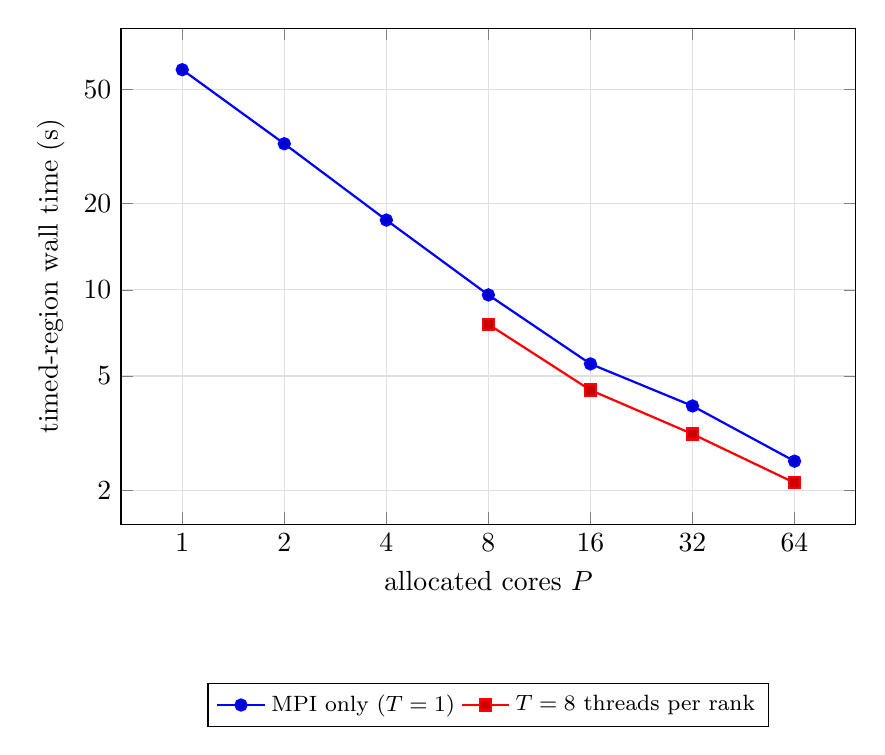
\begin{tikzpicture}
\begin{axis}[width=0.9\columnwidth, height=0.65\columnwidth, xlabel={allocated cores $P$}, ylabel={timed-region wall time (s)}, xmode=log, log basis x=2, log ticks with fixed point, ymode=log, ytick={1,2,5,10,20,50,100,200,500}, legend style={at={(0.5,-0.32)}, anchor=north, legend columns=2, font=\footnotesize}, legend cell align=left, grid=major, grid style={gray!25}]
\addplot+[mark=*, thick, error bars/.cd, y dir=both, y explicit] coordinates {(1,58.61) += (0,0.06977) -= (0,0.05899) (2,32.33) += (0,0.06327) -= (0,0.04105) (4,17.51) += (0,0.02666) -= (0,0.02227) (8,9.596) += (0,0.02178) -= (0,0.01817) (16,5.512) += (0,0.01523) -= (0,0.001253) (32,3.932) += (0,0.005636) -= (0,0.000128) (64,2.523) += (0,0.0267) -= (0,0.02405)};
\addlegendentry{MPI only ($T=1$)}
\addplot+[mark=square*, thick, error bars/.cd, y dir=both, y explicit] coordinates {(8,7.575) += (0,0.001504) -= (0,0.008238) (16,4.466) += (0,0.001819) -= (0,0.01937) (32,3.138) += (0,0.0159) -= (0,0.01573) (64,2.121) += (0,0.04136) -= (0,0.002554)};
\addlegendentry{$T=8$ threads per rank}
\end{axis}
\end{tikzpicture}
\caption{Strong-scaling runtime. $N=10^{6}$, median of repetitions; serial Barnes--Hut baseline on the same CPU model and build. Bars: fastest to slowest repetition. Vanda job 1528774: all 64 cores of Gold 6438N node IN-008, 3 interleaved repetitions.}
\label{fig:strong-runtime}
\end{figure}
